%%%%%%%%%%%%%%%%%%%%%%%%%%%%%%%%%%%%%%%%%%%%%%%%%%%%%%%%%%%%%%%%%%%%%%%%%%%%%%%%
\chapter{Evaluation}
\label{sec:eval}
%%%%%%%%%%%%%%%%%%%%%%%%%%%%%%%%%%%%%%%%%%%%%%%%%%%%%%%%%%%%%%%%%%%%%%%%%%%%%%%%

We evaluated four aspects of our system: \textbf{(1)} the utility and
simplicity of the policy language, %\textbf{(2)} the storage overhead of trusted capsules, 
\textbf{(2)} latency at the system call layer,
and \textbf{(3)} the overhead associated with different policies. %perceived latency at the application layer.

All performance evaluations were performed on our HiKey development board. 
%For the evaluation we used real file types %and applications,
% including JPEG/GpicView image viewer, TXT/Leafpad, and PDF/Evince PDF reader.

%% To interact with these data types, we used GpicView as our image
%% editor, VLC as our video player, LibreOffice writer as our document
%% editor and Evince as our PDF reader.
 
%%%%%%%%%%%%%%%%%%%%%%%%%%%%%%
\section{Policy language}
%%%%%%%%%%%%%%%%%%%%%%%%%%%%%%

In our policy language evaluation we aimed to answer two questions: is
the policy language adequate for expressing useful policies? And, are
these policies easy to express?

We answered our first question by writing trusted capsule policies for
the example use-cases from Section~\ref{sec:new-policies}. For our second
question, we measured the LOC for each policy that we wrote and show
the result in Table~\ref{policy-loc}.

The ability to easily express complex policies tersely is important
both as a proxy of simplicity and to bound the memory overhead of the
Lua interpreter in the secure world. We found that with a few lines of
code we were to express complex policies such as redaction and
revocation.

% We focus on two such policies. The first policy is used in the context
% of a sensitive merger document. We highlight one component of the
% policy, the system-level redaction policy in
% Figure~\ref{fig:merger_policy}.  This policy redacts all data within
% the byte offsets specified by \textit{redact\_sensitive}. These byte
% offsets were translated by a policy pre-processor from
% \textit{$<Sensitive>$} XML-like tags used to define the merger
% document. This redaction only occurs if the document is opened outside
% of the office as determined by the GPS coordinates.  The original data
% is replaced with the character defined by \textit{replace\_char}.

% We show the results in Figure~\ref{fig:redaction}.

%%%%%%%%%%%%%%%%%%%%%
%% \begin{figure}
%%   \centering
%%   \begin{subfigure}{\columnwidth}
%%   	\includegraphics[width=8cm, height=4cm]{../Images/non_redact.jpg}
%% 	\caption{Unredacted merger document.}
%% 	\label{fig:unredacted}
%%   \end{subfigure}\hfill
%%   \begin{subfigure}{\columnwidth}
%%   	\includegraphics[width=8cm, height=4cm]{../Images/redact.jpg}
%% 	\caption{Redacted merger document.}
%% 	\label{fig:redacted}
%%   \end{subfigure}\hfill 
%%   \caption{Before vs. after redaction.}
%%   \label{fig:redaction}
%%   % \vspace{-1em}
%% \end{figure}
%%%%%%%%%%%%%%%%%%%%%/

% The second policy is for photos stored in the cloud. The policy, shown
% in Figure~\ref{fig:image_policy}, allows only devices provisioned
% with the role-based identity ``Kate'' to access the photo. As described
% previously, with trusted capsules, an attacker who gains access to
% photos will not be able to access the capsule contents. On every
% \textit{open} system call, the monitor checks with the policy
% coordinator for updates to a remote state (line 7 in
% Figure~\ref{fig:image_policy}). If the remote server returns
% \textit{true}, the photo is deleted from the device.

% For these and other policies we found that the Lua policy interpreter
% needed less than 2KB of allocated memory.

%% However, while writing our trusted capsule policies, we discovered
%% some gaps in usability. For example, our Lua policy understands time
%% as an integer since January 1, 1970. Converting dates to such an
%% integer may be confusing and awkward. Currently we are exploring a
%% more feature-rich policy processor that would translate between more
%% human-friendly policy inputs to our Lua policy, however this is
%% outside the scope of the current work.

%%%%%%%%%%%%%%%%%%%%%%%%%%%%%%%%%
\begin{table}[h!]
\centering
{\small
\begin{tabular}{|l|c|}
\hline
\textbf{Policy}          & \textbf{LOC} \\ \hline\hline
Location Based Access & 30  \\ \hline
% Location Based Redaction (Using Lua String funcs)    & 63  \\ \hline
Location Based Redaction    & 45  \\ \hline
Content Distribution     & 28  \\ \hline
\end{tabular}
}
\caption{LOC for example policies from Section~\ref{sec:new-policies}.}
\label{policy-loc}
\end{table}
%%%%%%%%%%%%%%%%%%%%%%%%%%%%%%%%%

% TODO Have it import the file from a code directory.
% \begin{figure}
% \begin{lstlisting}[basicstyle=\tiny,linewidth=\columnwidth,xleftmargin=0.1\columnwidth,tabsize=2,numbers=left,breaklines=true,language={Python}]

% %\begin{lstlisting}%[caption={Sensitive Merger Document Policy.}]
% ...
% replace_char = "#"
% redact_sensitive = {45379, 45393, 45532, 45549, 45705, 45726, 45880, 45905, 46081, 46094, 46178, 46185, 46293, 46309, 46380, 46385, 46449, 46458, 46528, 46533, 46606, 46609, 46676, 46682, 46768, 46769, 46835, 46844, 46953, 46963, 47124, 47141, 47225, 47235, 47343, 47348, 47419, 47427, 47491, 47496, 47571, 47586, 47659, 47662, 47729, 47735, 47821, 47822, 47888, 47897, 48006, 48018, 48682, 48684, 48751, 48757, 48843, 48847, 49003, 49008, 49705, 49715, 49926, 49928, 50077, 50079, 50136, 50139, 50950, 50957, 51078, 51080, 51266, 51268, 51325, 51328, 52810, 52823, 54542, 54559};
% redact = {};
% ...
% -- READ
% elseif op == 1 then
% 	local long, lat = getgps();
% 	if((lat - 2130 >= 10) or (2130 - lat >= 10)) or ((lat - 22223 >= 10) or (22223-lat >= 10 )) then
% 		redact = redact_sensitive;
% 	end
% ...
% \end{lstlisting}
% \caption{Sensitive merger document policy.}
% \label{fig:merger_policy}
% \end{figure}

% \begin{figure}
% \begin{lstlisting}[basicstyle=\tiny,linewidth=\columnwidth,xleftmargin=0.1\columnwidth,tabsize=2,numbers=left,breaklines=true,language={Python}]

% %\begin{lstlisting}[caption={Private Image Policy},language={Python},breaklines=true,linewidth=\columnwidth]
% ...
% if getlocalstate( "cred" ) ~= "kate" then
% 	res = false;
% end
% -- OPEN
% if op == 0 then
% 	view_status == getserverstate( "delete?" );
% 	if ( view_status == "true" ) then
% 		delete();
% 	end
% ...
% \end{lstlisting}
% \caption{Private image policy.}
% \label{fig:image_policy}
% \end{figure} 


% %%%%%%%%%%%%%%%%%%%%%%%%%%%%%%
% \subsection{Storage overhead}
% %%%%%%%%%%%%%%%%%%%%%%%%%%%%%%

% Converting regular data into trusted capsules incurs storage overhead
% that is proportional with the policy size. We evaluate
% the associated overhead for different types of data.

% %%%%%%%%%%%%%%%%%%%%%%%%%%%%%%%%%%%%%%%%%%%%
% \begin{table}
% \begin{center}
% {\small
% \begin{tabular}{|l||*{3}{r|}}\hline
% %\backslashbox{Privilege}{World}
% &\makebox{\textbf{Data (KB)}}&\makebox{\textbf{Capsule (KB)}}&\makebox{\textbf{Overhead}}\\\hline\hline
% PDF Doc&137.34KB&139.38KB&1.42\%\\\hline
% JPEG Image&204.10KB&207.00KB&1.42\%\\\hline
% MP4 Video&4142.40KB&4175.94KB&0.80\%\\\hline
% LibreOffice Doc&54.80KB&56.70KB&3.47\%\\\hline
% \end{tabular}
% }
% \caption{Storage overhead for test data files.}
% \label{Tbl-StorageOverhead}
% \end{center} 
% \end{table}
% %%%%%%%%%%%%%%%%%%%%%%%%%%%%%%%%%%%%%%%%%%%%

% Table~\ref{Tbl-StorageOverhead} lists the storage overhead for a PDF,
% JPEG, MP4, and FODT files used in our evaluation. These data types were
% converted to trusted capsules with 4KB chunk sizes. We found the
% storage overhead to be negligible.

%%%%%%%%%%%%%%
\section{System call microbenchmarks}
%%%%%%%%%%%%%%


\begin{figure}[t]
  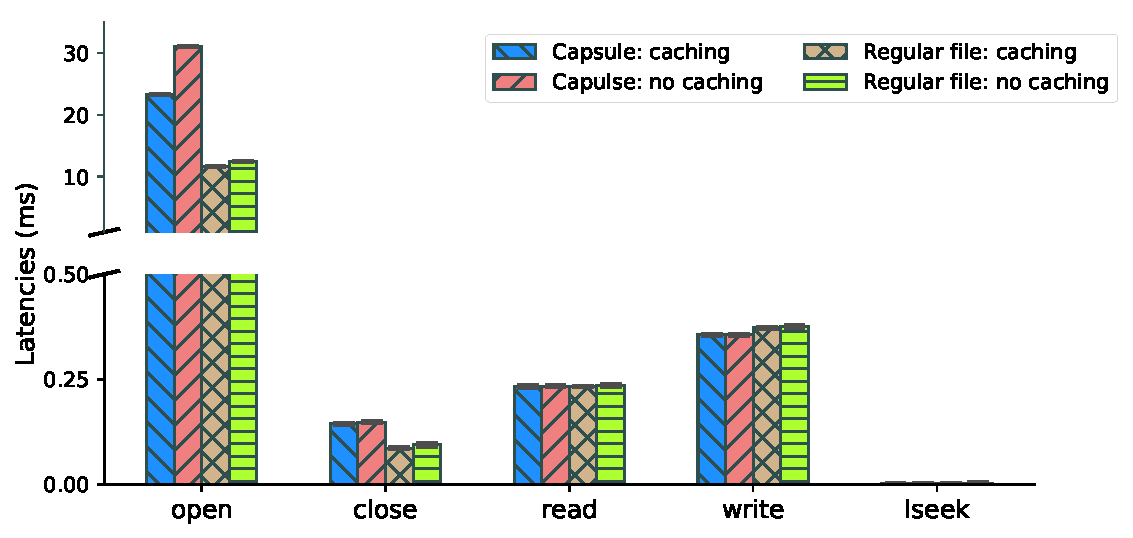
\includegraphics[width=8cm,height=4cm]{fig/latencies.pdf}
  \caption{Average system call latency}
  \label{fig:latencies}
\end{figure}

\begin{figure}[t]
  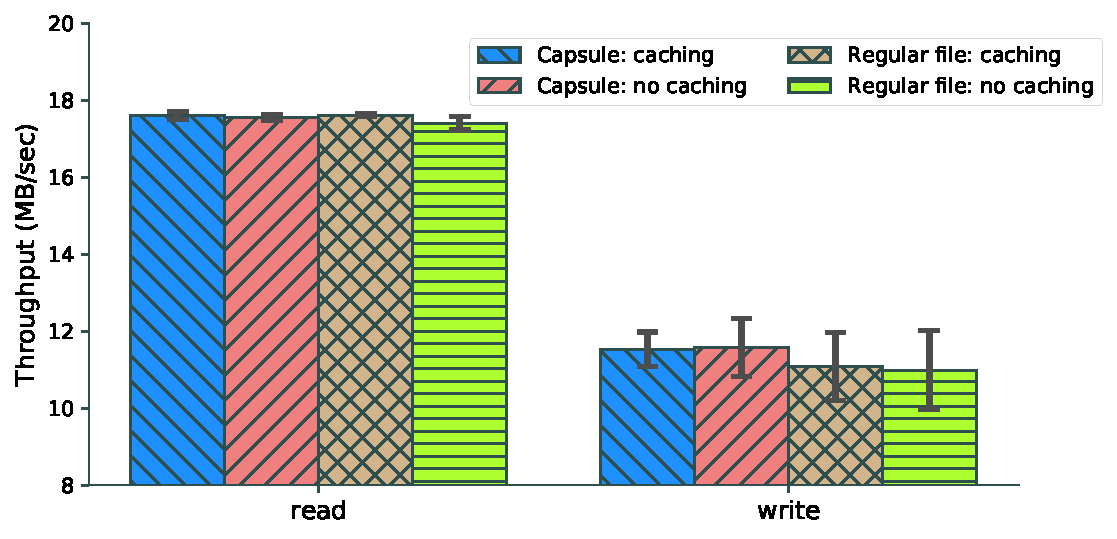
\includegraphics[width=8cm,height=4cm]{fig/rw_throughput.pdf}
  \caption{Throughput of Read and Write operations to a capsule}
  \label{fig:rw_throughput}
\end{figure}


In considering system call level microbenchmarks, we focus on three
questions.\\

\textbf{Are operations on regular files affected?} 
We measured the latency of filesystem operations for a regular file and a capsule. Since our system is based on FUSE, we evaluate the performance of the Trusted Capsule system by comparing against system call latencies for a regular file on the same mountpoint.

% We measured the
% performance of system call operations with and without the system call
% interceptor for both latency and throughput under similar conditions.
%Operations on regular data represents the fast path in our interceptor. 
We found that the performance of system calls on regular data is not impacted, except for \textit{open} syscall. 
This is due to the overhead of checking whether the target file is a trusted capsule. \\
%In addition, once a process
%has accessed a trusted capsule, write throughput on regular data also decreases linearly with
%number of trusted capsule accessed by that process due to the need to evaluate each trusted capsule's 
%declassify policies. 

\textbf{What is the latency and throughput of the system calls we
  intercept for operations on trusted capsules?} We measured the
latency and throughput of syscall operations on trusted capsules.  For
latency measurements, we measured the end-to-end time for a syscall
and averaged over 1000 runs.  For throughput measurements, we randomly
read and wrote 4KB of data to a trusted capsule for 10 seconds. To get an estimate of performance on the first use, we repeat the experiment with a cold cache achieved by dropping the page cache. 
For each test trusted capsule, we attached an empty null policy that always evaluated to true.  We present our results in Figure~\ref{fig:latencies} and ~\ref{fig:rw_throughput}.

The latency for \texttt{open} and \texttt{close} operations for a capsule present a prominent spike when compared to the operations on regular files. This is expected since our current prototype interposes on only these operations. An \texttt{open} operation on a null-policy capsule (warm cache) completes in 23 milliseconds compared to the 11.7 milliseconds for a regular file. The close operation on a capsule completes in  144 microseconds as compared to  86 microseconds for a regular file. 

The observed altency spike is more pronounced for \texttt{open} than for \texttt{close}. We understand this to be a direct result of the greater number of steps that have to happen in TrustZone to initialize the Trusted Application, which do not need to be done  while servicing a capsule close. 

We were able to achieve 17.59MB/s throughput for reading and 11.52MB/s throughput for writing to a no-op capsule on a warm cache. This is comparable to the read (17.6 MB/s) and write throughput (11.1 MB/s) achieved for a regular file when accessed in the same experimental setup. When the same experiments were repeated for a cold cache, the throughput drops marginally.

The read and write throughputs for a capsule, as compared to a normal
file, were expected to be nearly identical. This is expected in our
system since all reads and writes to a capsule gets directed to a
shadow file, which is treated like a regular file in FUSE.


% While we initially expected some impact to read and write performance at smaller chunk sizes, our
% results showed otherwise. We believe this may be due the fact that the cost of extra round trips between
% normal and secure world to fetch the same quantity of data is not significant overall.
% We also incur significant costs for \textit{open} syscall, especially at larger file sizes. 
% %Again, chunk size has little impact on performance. 
% While we do not expect \textit{open} syscall to be called often by applications 
% that interact with trusted capsule, its poor performance nevertheless requires further optimization. In our 
% current implementation, an \textit{open} syscall makes a pass over the entire data of the trusted capsule
% to validate the trusted capsule contents against its hash. This results in longer latencies as the file size
% increases. As can be seen, we were able to obtain reasonable results for \textit{open} calls on file sizes that
% were less than 100KB. However this latency increases dramatically for larger file sizes. 
% %In the future, we plan to explore possible optimizations. 


%For throughput, 
%we use 4KB request sizes as this is the granularity that most applications 
%read/write~\cite{evalpaper,filenotafile}. The throughput was run over a 10 second period.

%\begin{figure}[h!]
%	\includegraphics{../Graphs/Microbenchmarks_Latency.pdf}
%	\caption{The average latency per operation on a regular 1M file in varying system state (load and interceptor) with 95\% error bars.}
%	\label{micro_latency}
%\end{figure}

%\begin{figure}[h!]
%	\includegraphics{../Graphs/Microbenchmarks_Throughput.pdf}
%	\caption{The throughput measured over a ten second period on a regular 1M file in varying system state (load and interceptor).}
%	\label{micro_throughput}
%\end{figure}

% %%%%%%%%%%%%%%%%%%%%%
% \begin{figure}
%   \centering
%   \begin{subfigure}{\columnwidth}
%   	\includegraphics[width=8cm, height=4cm]{../Graphs/Chunk_Size_Comparison_Latency.pdf}
% 	\caption{Average latency varied by chunk size. The bars represent 95\%.}
% 	\label{fig:chunksize_latency}
%   \end{subfigure}\hfill
%   \begin{subfigure}{\columnwidth}
%   	\includegraphics[width=8cm, height=4cm]{../Graphs/Chunk_Size_Comparison_Throughput.pdf}
% 	\caption{Throughput varied by chunk size.}
% 	\label{fig:chunksize_throughput}
%   \end{subfigure}\hfill 
%   \caption{System call performance varied by chunk size. Test trusted capsules had a data size of 1M.}
%   \label{fig:chunksize}
%   % \vspace{-1em}
% \end{figure}
% %%%%%%%%%%%%%%%%%%%%%/

% %%%%%%%%%%%%%%%%%%%%%
% \begin{figure}
%   \centering
%   \begin{subfigure}{\columnwidth}
%   	\includegraphics[width=8cm, height=4cm]{../Graphs/File_Size_Comparison_Latency.pdf}
% 	\caption{Average latency varied by file size. The bars represent 95\%.}
% 	\label{fig:filesize_latency}
%   \end{subfigure}\hfill
%   \begin{subfigure}{\columnwidth}
% 	\includegraphics[width=8cm, height=4cm]{../Graphs/File_Size_Comparison_Throughput.pdf}
% 	\caption{Throughput varied by file size.}
% 	\label{fig:filesize_throughput}
%   \end{subfigure}\hfill 
%   \caption{System call performance varied by file size. Test trusted capsules created using 4KB chunk size.}
%   \label{fig:filesize}
%   % \vspace{-1em}
% \end{figure}
% %%%%%%%%%%%%%%%%%%%%%/

%\textbf{Tainted Processes.} \ac{Add better explanation of what this is showing.} We start the a 
%process. It sequentially opens each of our 
%use case capsules. Then we call write() on a regular file with 4KB request sizes at random
%offsets 10000 times. 

%Opened three different capsules with no-op policies: \ac{file size/chunk size per capsule here}.

%We see large degradation of the read throughput based on the number of capsules open. The write %throughput with no capsules open is about 2.0 MB/sec, once one capsule is open, the throughput drops to %0.5 MB/sec. 

% \begin{figure}[h!]
% 	\includegraphics{../Graphs/Tainted_Process.pdf}
% 	\caption{The throughput cost of having multiple capsules open while accessing a regular file.}
% 	\label{tainted_process}
% \end{figure}

% \textbf{What is the contribution of various aspects of the trusted
%   capsule monitor to per-operation latency overhead?} We evaluated the
% cost of the (1) normal world data monitor components (interceptor and
% linuxdriver), (2) world switch, (3) hashing, (4) encryption, (5)
% secure storage operations, (6) direct file system operations and (7)
% policy engine initialization.  We average our results over 100
% iterations of the same system call. Our test capsule had an empty null
% policy and used 4KB chunksize and consisted of 1MB of data. We show
% the results for (3)-(7) in
% Figure~\ref{fig:1M_4KB_breakdown_cycles}. We measured costs of these
% components end-to-end. For example, a secure storage operation in
% Figure~\ref{fig:1M_4KB_breakdown_cycles} would include the cost of
% world switches, userspace and kernel space boundary crossings, copying
% data between layers of the software stack and RPCs. All measurements
% are based on a 1.2 MHz monotonic counter.

% We found accessing secure storage to be an extremely expensive operation, accounting for a large number of cycles. This occurs when 
% policy evaluation needs to access state and on instantiation of the trusted capsule session when the cryptographic information is fetched.
% Further, the moderate costs associated with direct file system operations is in-line with
% our observation that decreasing chunk size (increasing the number of direct file system operations) did not affect performance 
% extensively. Surprisingly, encryption and hashing was not as a significant component of the overall cost as we thought. 
% Further, initializing the Lua interpreter, the normal world data monitor components (interceptor and
% linuxdriver) and world switching represented marginal costs. We measured the cost of both the normal world data monitor components and 
% evaluated the null policy to be few dozen cycles and a world switch to cost only a single cycle. 

% Perhaps the most interesting observation is that all these aspects (1)
% to (7) combined accounted for only $\sim$30\% of total cost of any
% syscall operation. These operations represent all the transitions that
% may occur between the trusted application and the remainder of the
% software stack (normal world components, OP-TEE OS, etc.), except for
% memory allocations (both between secure and normal world, and between
% userspace and kernel space within the secure world) and trusted
% application code. This leads us to believe that a significant portion
% of the slowdown is due to memory management across the stack and the
% in-memory copies and loops in the trusted application.

% To further evaluate the impact of world switch overhead, we measured the number of world switches for each operation. We broken down the
% world switch for different purposes. For any operation, we found that it required at most $\sim$100 world switches at a cost of 1-2 cycles per
% world switch. We make an interesting observation that most world switches are used to handle RPCs and their associate shared memory 
% allocations. 

% %%%%%%%%%%%%%%%%%%%%%
% \begin{figure}
%   \centering
%    \begin{subfigure}{\columnwidth}
%     \includegraphics[width=8cm, height=4cm]{../Graphs/Counter_Cycles_Breakdown_test_1M_NULL_4KB.pdf}
% 	\caption{Operations.}
% 	\label{fig:1M_4KB_breakdown_cycles}
%   \end{subfigure}\hfill 
%   \begin{subfigure}{\columnwidth}
%   	\includegraphics[width=8cm, height=4cm]{../Graphs/World_Switches_Breakdown_test_1M_NULL_4KB.pdf}
% 	  \caption{World Switches.}
% 	\label{fig:1M_4KB_breakdown_switches}
%   \end{subfigure}\hfill
%   \caption{Breakdown of number of cycles spent performing specific operations and number of world switches for specific purpose.}
%   \label{fig:1M_4KB_breakdown}  
%   % \vspace{-1em}
% \end{figure}
% %%%%%%%%%%%%%%%%%%%%%/

% \begin{figure}[h!]
	
% \end{figure}

% \begin{figure}[h!]
	
% \end{figure}

\section{Policy Performance Evaluation}

% We evaluate the performance of our trusted capsules at the macro-level
% directly with unmodified applications. We investigated how the
% overhead incurred by trusted capsules at the system call level impacts
% performance at the application level. For this purpose we used our use
% case trusted capsules.

In this section we present our preliminary findings on the impact that
policies of varying complexity have on the performance of the
system. %% We also present our past experience with making the older
%% system work with unmodified applications and the impact on the
%% perceived application slowdown.

To measure the overhead associated with the policy execution, we
compare the latency microbenchmarks for \texttt{open} operations for a
policy containing capsule, normalized with respect to the latency for
opening a null-policy capsule. These results are presented in
Figure~\ref{fig:policy_latency}. There is a sharp increase in the
latency when there is a non-null policy being evaluated, and this
latency increases with the complexity of the policy.

Figure~\ref{fig:policy_latency} compares two policies: a redaction
policy that redacts sensitive tags without performing other checks and
a local time based redaction policy, which performs redaction based on
the epoch value obtained from the device. The redaction policy uses
the \texttt{redact()} API from Table~\ref{Tbl:lua_ext}, while the Time
based redact policy uses the \texttt{redact()} API as well as well as
the \texttt{getTime()} API. This extra work to service an open request
is evident from Figure~\ref{fig:policy_latency}.

%%%%%%%%%%%%%%%%%%%%%%%%%%%%%%%%%%%%%%%%%%%%%%%%%%%%%%%%
\begin{figure}[t]
    \centering
    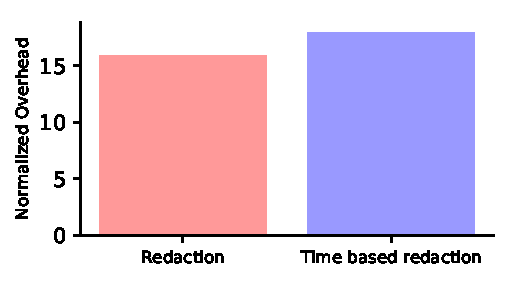
\includegraphics[width=8cm,height=4cm]{fig/policy_latencies.pdf}
    \caption{Normalized latency of servicing an \texttt{open} for different policies with respect to the latency to service a null-policy capsule open request. }
    \label{fig:policy_latency}
\end{figure}
%%%%%%%%%%%%%%%%%%%%%%%%%%%%%%%%%%%%%%%%%%%%%%%%%%%%%%%%


%% \begin{table*}[t]
%% \begin{center}
%% {\small
%% \begin{tabular}{|l|l|l|*{3}{r|}}\hline
%% %\backslashbox{Privilege}{World}
%% \makebox{\textbf{Data Type}}&\makebox{\textbf{Application}}&\makebox{\textbf{Interactions}}&\makebox{\textbf{Regular Data}}&\makebox{\textbf{Null Policy}}&\makebox{\textbf{Use-Case Policy}}\\\hline\hline
%% PDF Doc&Evince&Open document&0.87s&3.20s&110.40s\\\hline
%% JPEG Image&Gpicview&Open image, rotate, save&0.45s/0.23s/0.17s&6.45s/0.88s/3.43s&20.23s/1.43s/11.38s\\\hline
%% MP4 Video&VLC&Buffering time before playing&3.21s&3.92s&25.72s\\\hline
%% LibreOffice Doc&LibreOffice Writer&Open document&1.63s&12.42s&21.67s\\\hline
%% \end{tabular}
%% }
%% \caption{Application level performance as observed from first prototype's evaluation}
%% \label{Tbl-Macro-performance}
%% \end{center} 
%% \end{table*}


%%  We believe that such performance degradations can be
%% mitigated with more efficient policy code, for example policies that
%% run at coarser granularity or use caching to mitigate expensive
%% checks.
